% This is "sig-alternate.tex" V2.1 April 2013
% This file should be compiled with V2.5 of "sig-alternate.cls" May 2012
%
% This example file demonstrates the use of the 'sig-alternate.cls'
% V2.5 LaTeX2e document class file. It is for those submitting
% articles to ACM Conference Proceedings WHO DO NOT WISH TO
% STRICTLY ADHERE TO THE SIGS (PUBS-BOARD-ENDORSED) STYLE.
% The 'sig-alternate.cls' file will produce a similar-looking,
% albeit, 'tighter' paper resulting in, invariably, fewer pages.
%
% ----------------------------------------------------------------------------------------------------------------
% This .tex file (and associated .cls V2.5) produces:
%       1) The Permission Statement
%       2) The Conference (location) Info information
%       3) The Copyright Line with ACM data
%       4) NO page numbers
%
% as against the acm_proc_article-sp.cls file which
% DOES NOT produce 1) thru' 3) above.
%
% Using 'sig-alternate.cls' you have control, however, from within
% the source .tex file, over both the CopyrightYear
% (defaulted to 200X) and the ACM Copyright Data
% (defaulted to X-XXXXX-XX-X/XX/XX).
% e.g.
% \CopyrightYear{2007} will cause 2007 to appear in the copyright line.
% \crdata{0-12345-67-8/90/12} will cause 0-12345-67-8/90/12 to appear in the copyright line.
%
% ---------------------------------------------------------------------------------------------------------------
% This .tex source is an example which *does* use
% the .bib file (from which the .bbl file % is produced).
% REMEMBER HOWEVER: After having produced the .bbl file,
% and prior to final submission, you *NEED* to 'insert'
% your .bbl file into your source .tex file so as to provide
% ONE 'self-contained' source file.
%
% ================= IF YOU HAVE QUESTIONS =======================
% Questions regarding the SIGS styles, SIGS policies and
% procedures, Conferences etc. should be sent to
% Adrienne Griscti (griscti@acm.org)
%
% Technical questions _only_ to
% Gerald Murray (murray@hq.acm.org)
% ===============================================================
%
% For tracking purposes - this is V2.0 - May 2012

\documentclass{sig-alternate-05-2015}
\usepackage{pdfpages}

% Use Roman numerals for tables
\renewcommand{\thetable}{\Roman{table}}

\begin{document}

% Copyright
\setcopyright{acmcopyright}
%\setcopyright{acmlicensed}
%\setcopyright{rightsretained}
%\setcopyright{usgov}
%\setcopyright{usgovmixed}
%\setcopyright{cagov}
%\setcopyright{cagovmixed}


% DOI
% \doi{10.475/123_4}

% ISBN
% \isbn{123-4567-24-567/08/06}

%Conference
% \conferenceinfo{PLDI '13}{June 16--19, 2013, Seattle, WA, USA}

% \acmPrice{\$15.00}

%
% --- Author Metadata here ---
% \conferenceinfo{WOODSTOCK}{'97 El Paso, Texas USA}
%\CopyrightYear{2007} % Allows default copyright year (20XX) to be over-ridden - IF NEED BE.
%\crdata{0-12345-67-8/90/01}  % Allows default copyright data (0-89791-88-6/97/05) to be over-ridden - IF NEED BE.
% --- End of Author Metadata ---

\title{The Physical Benefits of VR games}
% \subtitle{[Extended Abstract]
% \titlenote{A full version of this paper is available as
% \textit{Author's Guide to Preparing ACM SIG Proceedings Using
% \LaTeX$2_\epsilon$\ and BibTeX} at
% \texttt{www.acm.org/eaddress.htm}}}
%
% You need the command \numberofauthors to handle the 'placement
% and alignment' of the authors beneath the title.
%
% For aesthetic reasons, we recommend 'three authors at a time'
% i.e. three 'name/affiliation blocks' be placed beneath the title.
%
% NOTE: You are NOT restricted in how many 'rows' of
% "name/affiliations" may appear. We just ask that you restrict
% the number of 'columns' to three.
%
% Because of the available 'opening page real-estate'
% we ask you to refrain from putting more than six authors
% (two rows with three columns) beneath the article title.
% More than six makes the first-page appear very cluttered indeed.
%
% Use the \alignauthor commands to handle the names
% and affiliations for an 'aesthetic maximum' of six authors.
% Add names, affiliations, addresses for
% the seventh etc. author(s) as the argument for the
% \additionalauthors command.
% These 'additional authors' will be output/set for you
% without further effort on your part as the last section in
% the body of your article BEFORE References or any Appendices.

\numberofauthors{5} %  in this sample file, there are a *total*
% of EIGHT authors. SIX appear on the 'first-page' (for formatting
% reasons) and the remaining two appear in the \additionalauthors section.
%
\author{
% You can go ahead and credit any number of authors here,
% e.g. one 'row of three' or two rows (consisting of one row of three
% and a second row of one, two or three).
%
% The command \alignauthor (no curly braces needed) should
% precede each author name, affiliation/snail-mail address and
% e-mail address. Additionally, tag each line of
% affiliation/address with \affaddr, and tag the
% e-mail address with \email.
%
% 1st. author
\alignauthor
Oona Kivelä \titlenote{Corresponding author}\\
    %    \email{trovato@corporation.com}
% 2nd. author
\alignauthor
Toni Kuosmanen 
% \email toni.kuosmanen@student.oulu.f
% 3rd. author
\alignauthor Timo Lämpsä
    %    \email{larst@affiliation.org}
\and  % use '\and' if you need 'another row' of author names
% 4th. author
\alignauthor Leevi Mustajärvi\\
% 5th. author
\alignauthor Joonas Soudunsaari\\
    %    \affaddr{NASA Ames Research Center}\\
    %    \affaddr{Moffett Field}\\
    %    \affaddr{California 94035}\\
    %    \email{fogartys@amesres.org}
}
% There's nothing stopping you putting the seventh, eighth, etc.
% author on the opening page (as the 'third row') but we ask,
% for aesthetic reasons that you place these 'additional authors'
% in the \additional authors block, viz.
% \additionalauthors{Additional authors: John Smith (The Th{\o}rv{\"a}ld Group,
% email: {\texttt{jsmith@affiliation.org}}) and Julius P.~Kumquat
% (The Kumquat Consortium, email: {\texttt{jpkumquat@consortium.net}}).}
% \date{30 July 1999}
% Just remember to make sure that the TOTAL number of authors
% is the number that will appear on the first page PLUS the
% number that will appear in the \additionalauthors section.
\maketitle
% \begin{abstract}
% This paper provides a sample of a \LaTeX\ document which conforms,
% somewhat loosely, to the formatting guidelines for
% ACM SIG Proceedings. It is an {\em alternate} style which produces
% a {\em tighter-looking} paper and was designed in response to
% concerns expressed, by authors, over page-budgets.
% It complements the document \textit{Author's (Alternate) Guide to
% Preparing ACM SIG Proceedings Using \LaTeX$2_\epsilon$\ and Bib\TeX}.
% This source file has been written with the intention of being
% compiled under \LaTeX$2_\epsilon$\ and .

% The developers have tried to include every imaginable sort
% of ``bells and whistles", such as a subtitle, footnotes on
% title, subtitle and authors, as well as in the text, and
% every optional component (e.g. Acknowledgments, Additional
% Authors, Appendices), not to mention examples of
% equations, theorems, tables and figures.

% To make best use of this sample document, run it through \LaTeX\
% and BibTeX, and compare this source code with the printed
% output produced by the dvi file. A compiled PDF version
% is available on the web page to help you with the
% `look and feel'.
% \end{abstract}


%
% The code below should be generated by the tool at
% http://dl.acm.org/ccs.cfm
% Please copy and paste the code instead of the example below. 
%
% \begin{CCSXML}
% <ccs2012>
%  <concept>
%   <concept_id>10010520.10010553.10010562</concept_id>
%   <concept_desc>Computer systems organization~Embedded systems</concept_desc>
%   <concept_significance>500</concept_significance>
%  </concept>
%  <concept>
%   <concept_id>10010520.10010575.10010755</concept_id>
%   <concept_desc>Computer systems organization~Redundancy</concept_desc>
%   <concept_significance>300</concept_significance>
%  </concept>
%  <concept>
%   <concept_id>10010520.10010553.10010554</concept_id>
%   <concept_desc>Computer systems organization~Robotics</concept_desc>
%   <concept_significance>100</concept_significance>
%  </concept>
%  <concept>
%   <concept_id>10003033.10003083.10003095</concept_id>
%   <concept_desc>Networks~Network reliability</concept_desc>
%   <concept_significance>100</concept_significance>
%  </concept>
% </ccs2012>  
% \end{CCSXML}

% \ccsdesc[500]{Computer systems organization~Embedded systems}
% \ccsdesc[300]{Computer systems organization~Redundancy}
% \ccsdesc{Computer systems organization~Robotics}
% \ccsdesc[100]{Networks~Network reliability}


%
% End generated code
%

%
%  Use this command to print the description
%
\printccsdesc

% We no longer use \terms command
%\terms{Theory}

\keywords{VR; Exergames; Heartrate;}

\section{INTRODUCTION AND MOTIVATION}
The aim of this study is to detect the physical benefits in virtual reality 
(VR) gaming. To get to the goal the heart rate of the subjects is going to 
be measured in rest and during the game. Also, subjects are interviewed about 
their exercise and gaming habits. There is also going to be questions about 
the VR game experience. The goal is to see whether VR games have physical 
effects to user and if user enjoys exercising with the VR game.

Motivation to exercise by exergames have been studied. Finkelstein et al. 
(2011) designed a game called Astrojumper which forces the user to move 
his/her whole body while playing. Player flies in outer space and swerve 
around, duck under and jump over virtual planets. They studied the 
effectiveness of this kind of game by measuring the heart rate before the 
game session and after the game session. One game session lasted 15 minutes. 
To get more information about the motivational part of the game they also 
asked the test users to fill pre- and post-questionnaires. Pre-questionnaire 
included more general information about user’s exercise habits and experiment 
with video games. In post-questionnaire the questions were focused on to the 
game session. It was shown that virtual reality games have strong potential 
to motivate to physical activity both adults and children.

Finkelstein et al. (2011) made their research seven years ago and the VR 
equipment are highly improved since then. In their Astrojumper study a user 
had a control backpack in his/hers back with many wires leading from there. 
The game setting in Astrojumper is highly different than what it is nowadays. 
The monitors are placed around the user while today user needs VR glasses with 
wireless control sticks. Movement trackers are on the forehead, wrists and 
waist in the Astrojumper. Finkelstein et al. (2011) had problems with heart 
rate measurements during the game session.

\section{RELATED WORK}
\subsection{Virtual reality games}
If the system consists a human operator, a human-machine interface and 
a computer it can be called a virtual environment. Environment has 
three-dimensional space where the objects are placed. 
\cite{national1995virtual}. Virtual reality games are characterized by high 
level of presence and immersion, or the feeling of really being a part 
of the virtual environment \cite{steuer1992defining}.

Adaptation of VR systems has been partly hampered by many users 
experiencing a set of symptoms similar to motion sickness. This set 
of symptoms is commonly called cybersickness. Possible symptoms include 
but are not limited to nausea, dizziness, headaches and fatigue. 
Studies have estimated that 30 \% - 80 \% percent of VR users 
experience these symptoms to some extent \cite{rebenitsch2016review}.

\subsubsection{HTC Vive, Oculus and Sony Playstation}
In recent years, many new consumer virtual reality systems have entered 
the market. Commonly these systems include an immersive head mounted 
display (HMD) and motion controllers. Popular examples of these systems 
include products such as Oculus Rift, HTC Vive or Playstation VR. Advanced 
head tracking and motion controllers combine to produce a high level of 
immersion and allow the user to explore and interact with their immediate 
surroundings in a natural fashion. Although Amazon sales rankings have 
recently shown a declining interest in VR devices \cite{vr_consumer}, 
millions of devices have been shipped worldwide.

\subsubsection{Exergames}
Exergame term is widely used when video games are played to promote 
physical activity \cite{oh2010defining}. Children are easier to motivate 
to exercise with a fun way and childhood obesity can be prevent by 
exergames \cite{staiano2013adolescent}. According to Staiano et al. (2013) 
children who were competitive exergames did not lose weight while 
cooperative “exergamers” did. Studies with elderly shows that with 
them the fun is not the driven force to play but the usefulness of 
the related physical and cognitive abilities is. \cite{chen2018acceptance}

Study conducted by Plante et al. (2003) found evidence that combining 
VR with physical exercise can boost the mood benefits associated with 
normal exercise. In the study people who were immersed in a virtual 
environment while riding an exercise bike generally reported feeling 
more energized and less tired than the people in the control group 
\cite{plante2003might}. 

Fitzgerald et al. (2010) have shown that exergames has been used successfully 
also in therapy. They used a wobble-board based on video game to motivate 
the patients. Their results show that patients are more motivated for 
training when comparing to those who does similar exercises at a class 
with a therapist. Dynamic stability in both test groups gained and there 
were no significant differences between groups. \cite{fitzgerald2010effects}

\subsection{Heart rate and exercise intensity}
Heart rate measurements have long been used to monitor exercise intensity 
\cite{achten2003heart}. A common way to represent exercise intensity 
using heart rate is to calculate the current heart rate as a percentage 
of the maximum heart rate: 

\begin{equation}\%HR = \frac{HR}{HR_{max}}\end{equation}

Although the maximum heart rate varies greatly between individuals, 
it can be estimated without measurement if the persons age is known:

\begin{equation}HR_{max} = 210 - 0.5 * age\end{equation}

Many different versions of the formulas exist, although none have been found 
to be very reliable \cite{robergs2002surprising}. Gulati et al. (2010) propose a slightly different age scaling factor of 0.88 for women.
as the most acceptable estimate of maximum heart rate. Gulati et al. \cite{gulati2005heart} 
propose a slightly different age scaling factor of 0.88 for women.

Another method used to gauge the exercise intensity is the heart rate reserve 
\cite{karvonen1957effects}). Instead of scaling the heart rate directly to the 
maximum heart rate, the subjects heart rate reserve is calculated using the formula:

\begin{equation}HR_{RESERVE} = HR_{MAX} - HR_{REST}\end{equation}

Relative heart rate can then be used to detect the changes in the heart rates. 
Relative heart rate is calculated with the following formula:

\begin{equation}HRR = \frac{HR - HR_{REST}}{HR_{RESERVE}} * 100\%\end{equation}

During training, different target heart rate zones can be set, depending on the 
goal of the exercise. For example, Fitdigits, a smart device based fitness application, 
suggests HRR values of over 50\% for light aerobic recovery and values of over 60\% 
for endurance training \cite{fitdigits}.  

\section{DESIGN}
To evaluate the potential health benefits, we chose two VR games available on the Steam 
platform. The two games were chosen based on their metabolic equivalent (MET) scores 
provided by VR Institute of Health and Exercise \cite{vrhealth_met}. The first game 
chosen was an arcade style archery simulation called QuiVR. VR Health Institute rates 
the game at 2.73 METs, roughly equivalent to walking or doing light housework. For the 
second game, we chose a more intense rhythm game called BeatSaber. In the game the player 
must cut moving colored blocks and dodge around obstacles. VR health institute gives the 
game an average METs score of 6.24, roughly equivalent of playing tennis or jogging. 
Our aim in choosing two games with different MET scores was twofold. First, we wanted to 
find out if even a game of modest activity could be considered exercise. Second, we wanted 
to see if a more active game be comparable to traditional physical exercise. 

We chose the users heart rate as the main measure of exercise intensity. For measuring the 
heartrate, we obtained two Fitbit Charge HR activity bracelets. The device measures the 
heart rate at an interval of five seconds. The measurements are stored on the device until 
they are synced to the Fitbit cloud service using a connected mobile phone. Afterwards, 
the heart rate data could be retrieved using a third-party application called Pulse Watch 
\cite{pulsewatch}. 

To compliment the heart rate data, we decided to also capture motion data from the VR 
game set. The set includes an HMD unit and two motion controllers. The position of each 
of these devices is tracked by two beacons. For logging this positional data, we 
prepared a simple program that could be ran parallel with the chosen games. While active, 
the program samples the device position and orientation at a rate of 5 Hz and outputs the 
data to a csv file. 

We prepared a multi-part interview to gain information if VR games increase exercise motivation. 
The first part of the interview dealt with participants gaming and exercise background and 
was held before the first game session. The second part of the interview was completed after 
first game session, and last part was after both sessions. Participants are asked to answer 
questions about their general background, exercising background, gaming background and about 
the VR game experience. 

\subsection{Cybersickness and heart rate}
As mentioned earlier, many VR users experience some degree of cybersickness. High levels 
of nausea can lead to increased heart rate without any physical activity \cite{nalivaiko2015cybersickness}. 
In order to find out if the observed increase in heart rate is caused by onset of cybersickness 
instead of exercise, we decided to include the standard Simulator Sickness Questionnaire 
(SSQ) \cite{kennedy1993simulator} as part of our survey. The SSQ, which was originally 
developed for military air simulation use, has been widely used in cybersickness research. 
The SSQ measures 16 different symptoms on a four-point scale. The symptoms are grouped to 
three different categories: oculomotor symptoms, disorientation, and nausea. From the raw 
data a score for each of the three main symptom categories and a total score can be calculated 
(SSQ-O, SSQ-D, SSQ-N, and SSQ-T respectively). SSQ was filled immediately after the participants 
had completed both game sessions.  Since nausea is the symptom mostly linked with increased 
heart rate, we paid special attention to the SSQ-N scores.

\section{EVALUATION}
\subsection{Evaluation plan}
Our VR gaming device which included HTC Vive visor, two motion controllers and two base 
stations which were set Ubicomp demo room inside Oulu university faculty of information 
technology and electrical engineering. We gathered 17 participants to play two different 
games. The experiments took place between 30.10 – 1.11.2018, during which a 30-minute 
time session was reserved for each participant. 

\begin{figure}
    \centering
    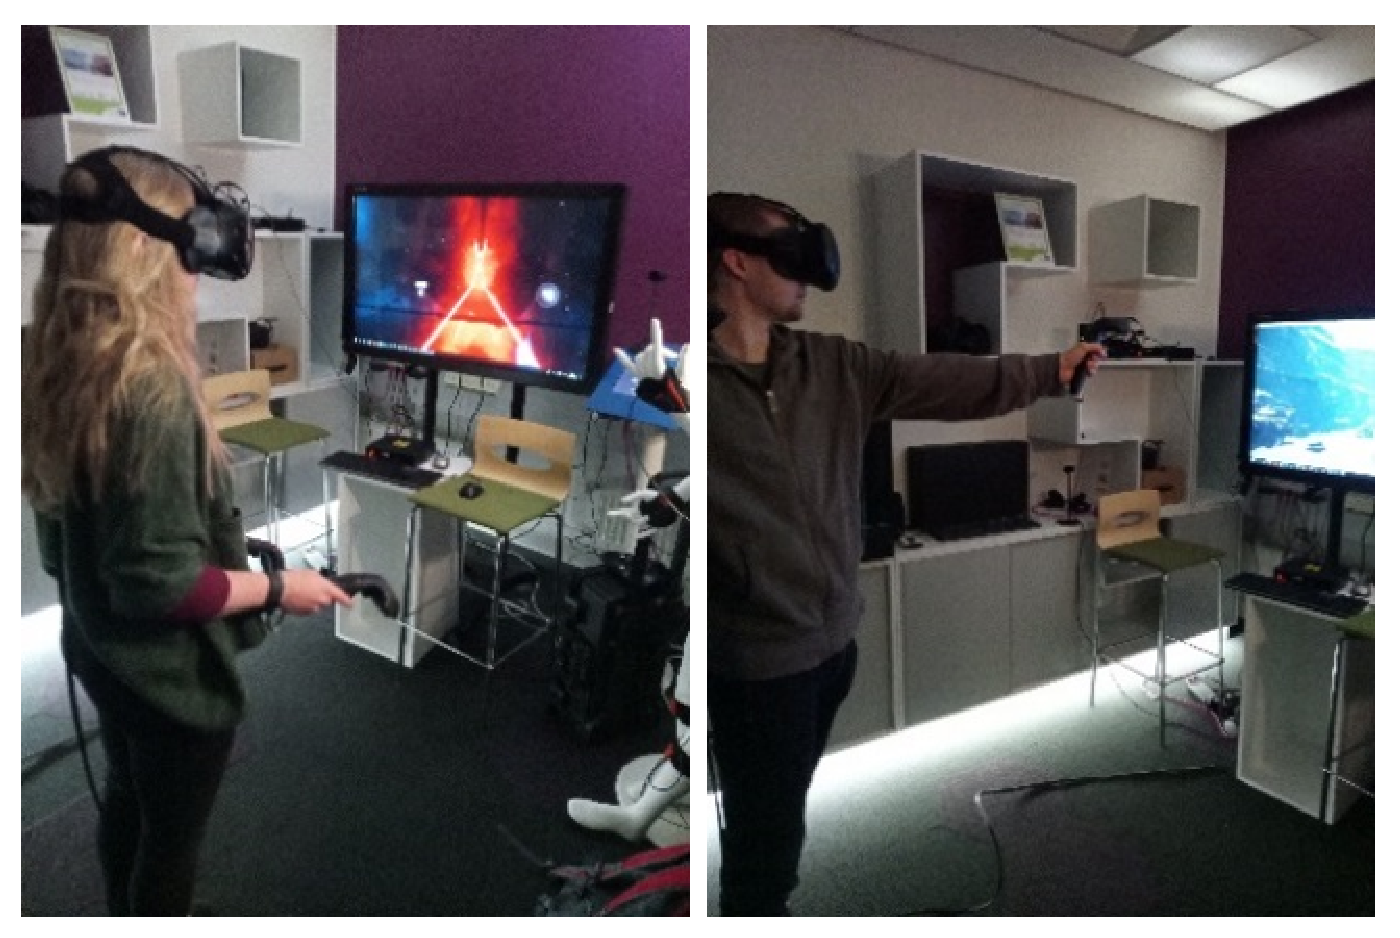
\includegraphics[width=0.45\textwidth]{players}
    \caption
        {
            Participants had two game sessions, each for 10 minutes. 
            Order of game sessions was randomly chosen. Participants played 
            BeatSaber and QuiVR games. 
        }
\end{figure}

At the beginning of their sessions the participant was sat down, and the Fitbit activity 
bracelet was attached to their wrist and the heart rate measurements started immediately. 
This was done in order to get an estimate of the participants resting heart rate.  
Participants were asked to fill a consent form (Attachment 1) and the first part of the 
survey. To protect the privacy of all the volunteers, each participant was assigned an 
ID number which was then used to connect heart rate, movement data and survey answers 
together. 

The order in which the games were played was alternated between participants. At the 
start of both gaming sessions, the participants were given a brief tutorial to get them 
accustomed to the controls. When the tutorial was completed, the motion logger was 
turned on and the actual gaming session was commenced. Both gaming sessions lasted for 
ten minutes (Figure 1). The start and end times were recoded, so that the heart rate 
data could be synchronized afterwards. After the first game session the participant was 
asked to rate the physical intensity of their game session. If their heart rate had 
increased noticeably, they were also given a small break so that the heart rate could 
climb down back to the levels observed before starting the first gaming session. 

The SSQ was administered immediately after the second gaming session had concluded. 
The participants were asked if they had any of the listed symptoms and if they did, 
they were asked to rate the severity of their symptoms on a four-point scale.  The 
final part of the survey, which dealt mainly with how the participant felt about VR 
based exercise based on their experience, was also filled. 

\subsection{Research data}
During the game session we gathered three types of data from test users. We gave 
them a Fitbit bracelet which measured heart rate in real time. We collected qualitative 
data from users by interviewing users before game session, after first game session and 
finally after second game session. We also had SSQ interview to participants. We gathered 
movement data from hand consoles and VR glasses via capture software which was run parallel 
to the VR game.

\subsubsection{Data from interviews}
During the first part of the survey, the participants were asked for some general background 
information. Participants age was recorded in order to calculate theoretical maximum 
heart rate. Gender was also recorded, but the low rate of women participants prevents data 
comparison between genders. Participants were asked to describe their weekly amount of physical 
exercise and how many hours a week they spend playing console or video games. Participants were 
also asked if they had used VR applications before. 

After first game session interview was continued by asking how user was feeling after the 
game. Users’ were also asked how intense they would rate the game session in a scale from 
one to five. After second game session participant was asked again how they feel, and 
how intense they would rate the game session. At the last part of the interview participant 
was asked whether he/she sees himself/herself playing VR games for exercise meaning and 
for fun in scale one to five. Whether participant would play virtual reality games in 
exercise context and would he/she recommend that to others in scale one to five. 
Participants had also a chance to say any comment about the whole experience. Results from 
interview are shown in Table I. Intensity of the game session results are shown in Figure 2.

\begin{table}
    \centering
    \caption
    {
        Survey results.\newline
        Q1: How many times a week you do sports? (at least 30 mins of exercising per time)\newline
        Q2: How many hours do you usually play computer games or console games in a week?\newline
        Q3: Could you see yourself playing virtual reality games more often just for fun?\newline
        Q4: Could you see yourself playing a virtual reality games more often for exercise purposes?\newline
        Q5: Would VR playing encourage you to exercise more?\newline
        Q6: Would you recommend VR gaming as an exercise for anyone?\newline
    }
    \begin{tabular}{c|c c c c c c} \hline
        % ID&How many times a week you do sports? (at least 30 mins of exercising per time)&How many hours do you usually play computer games or console games in a week?&Could you see yourself playing virtual reality games more often just for fun?&Could you see yourself playing a virtual reality games more often for exercise purposes?&Would VR playing encourage you to exercise more?&Would you recommend VR gaming as an exercise for anyone?\\ \hline
        ID&Q1&Q2&Q3&Q4&Q5&Q6 \\ \hline
        3&2&10&5&5&4&5\\
        4&3&0&5&3&3&3\\
        7&3&7&5&3&2&4\\
        8&4&0&4&4&2&2\\
        10&3&3&5&4&2&3\\
        12&4&1&4&2&4&5\\
        13&2&2&5&3&2&5\\
        16&3&25&5&1&1&2\\
        17&4&0&4&1&3&2\\
        18&5&4&4&1&1&2\\
        22&4&5&4&3&2&2\\
        23&2&5&5&3&4&2\\
        25&1&0&3&4&2&5\\
        26&1&30&5&4&3&3\\
        27&10&4&5&3&2&4\\
        29&3&0&5&4&4&4\\
        30&1&2&5&2&4&5\\ \hline
        Avg&3.2&5.8&4.6&2.9&2.6&3.4
    \end{tabular}
\end{table}

\begin{figure}
    \centering
    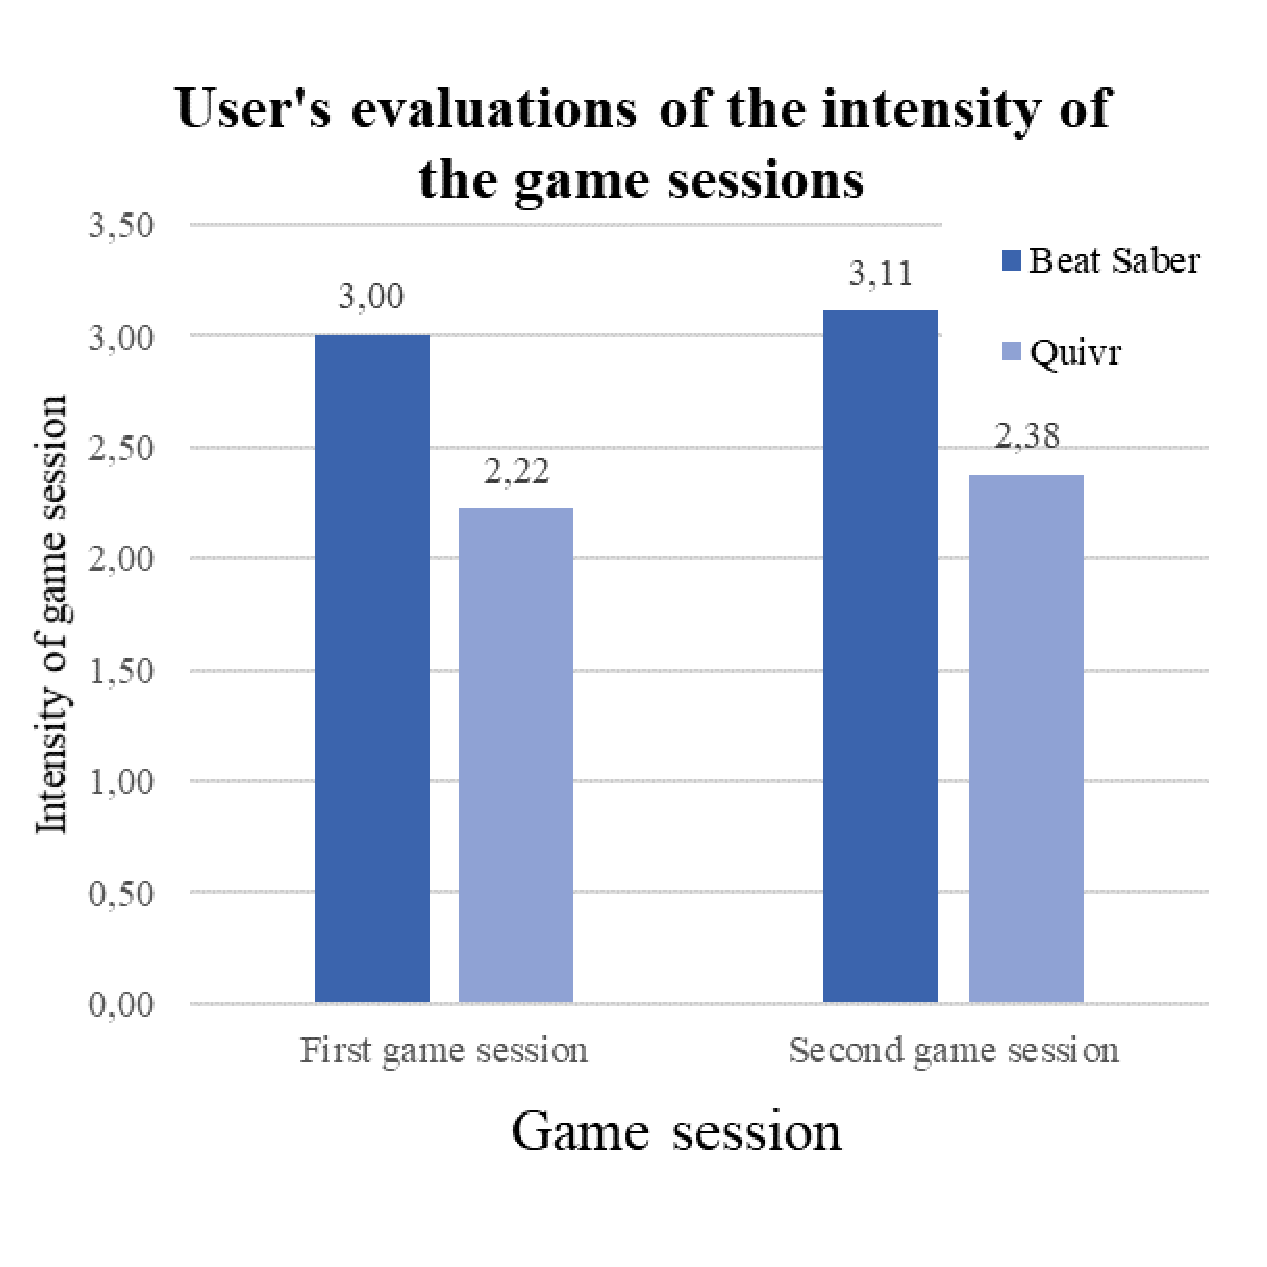
\includegraphics[width=0.45\textwidth]{intensity_evaluation}
    \caption
        {
            Users evaluation of intense of game session. Users, who played BeatSaber 
            first, evaluated the intense of the game session in average 3.00 in scale 
            one to five, and users playing QuiVR first 2.22. Users who played BeatSaber 
            in second game session evaluated the intense of the game in average 3.11, 
            and users who played QuiVR in second game session 2.58.
        }
\end{figure}

\begin{figure*}
    \centering
    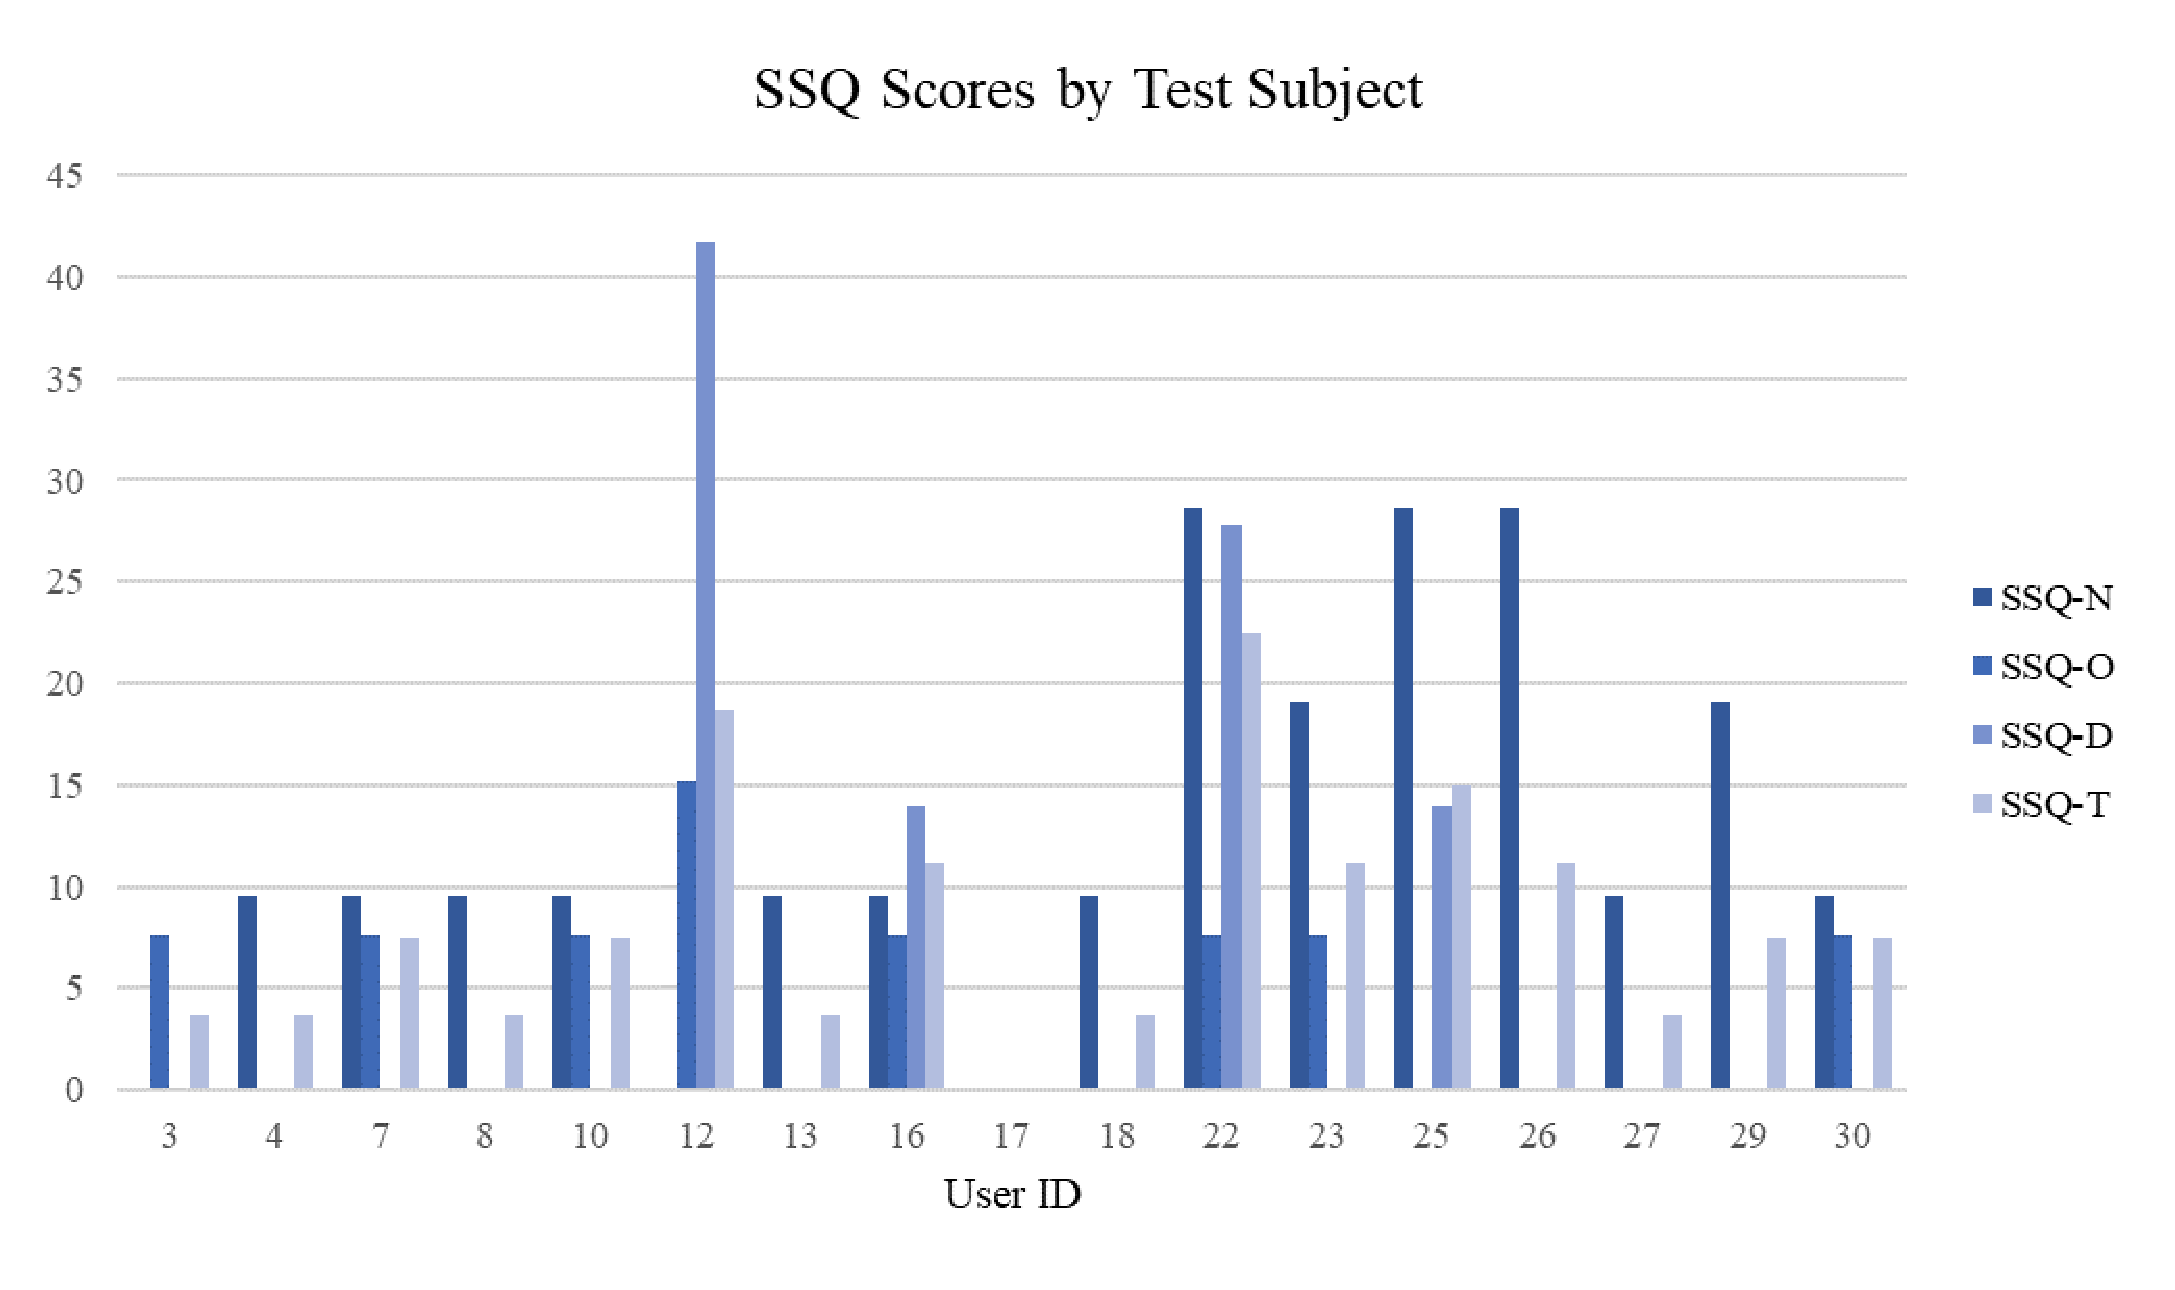
\includegraphics[width=0.80\textwidth]{ssq}
    \caption
        {
            Simulator sickness questionnaire results from each participant. 
            SSQ-N results shows weighted results of nausea symptoms, SSQ-O 
            results shows weighted results of oculomotor symptoms, SSQ-D 
            shows weighted results of disorientation symptoms and SSQ-T 
            shows total results.
        }
\end{figure*}

To ensure that the increase in subjects heart rate was not caused by the onset of cybersickness, 
we asked each subject to answer the simulator sickness questionnaire immediately after the second 
game session. The questionnaire consists of a list of sixteen symptoms associated with cybersickness. 
Simulator sickness questionnaire data was gathered from users after game session and the data is 
summarized to show three main symptom clusters of the questionnaire. Answers to these questions are 
ranked to be 0 if user don’t have the symptom, 1 if user feels slightly to have a symptom, 2 if user feels the symptom as moderate and 3 if user feels the symptom being severe. 
Different clusters are oculomotor (SSQ-O), disorientation (SSQ-D) and nausea (SSQ-N). SSQ-O 
includes the results about general feeling, fatigue, difficulty concentration, eye strain, 
difficulty focusing, blurred vision and headache. SSQ-D includes the results about difficulty 
focusing, nausea, “fullness of head”, blurred vision, dizziness with eyes open and closed, 
and vertigo. SSQ-N includes the results about general feeling, difficulty concentrating, 
nausea, stomach awareness, increased salivation, sweating and burping. SSQ total (SSQ-T) is 
calculated from the three clusters as a total value. Formulas used to get SSQ-O, SSQ-D, and 
SSQ-N scores are as follows:

\begin{equation}SSQ-O = \sum{O-cluster} * 7.58\end{equation}

\begin{equation}SSQ-D = \sum{D-cluster} * 13.92\end{equation}

\begin{equation}SSQ-N = \sum{N-cluster} * 9.54\end{equation}

And the total SSQ is calculated as the sum of the all the symptoms and multiplied with 3,74. 
Results are shown as a graph in Figure 2.

\subsubsection{Heart rate data}
Heart rate data was captured in real time by Fitbit bracelet. The bracelet 
measured the heart rate five seconds. The raw data was exported from Fitbit 
cloud storage using the PulseWatch application. Out of the 17 test users the 
data was successfully gathered from 14 participants. The data from three test 
subjects was lost due to connectivity issues with the Fitbit device. 

Participants maximum heart rate and relative heart rates were estimated using 
formulas 2, 3 and 4. Resting heart rate was measured from the participants while 
they were being interviewed for the first part of the survey. The average relative 
heart rates for both game sessions are shown in figure 3.  

\begin{figure}
    \centering
    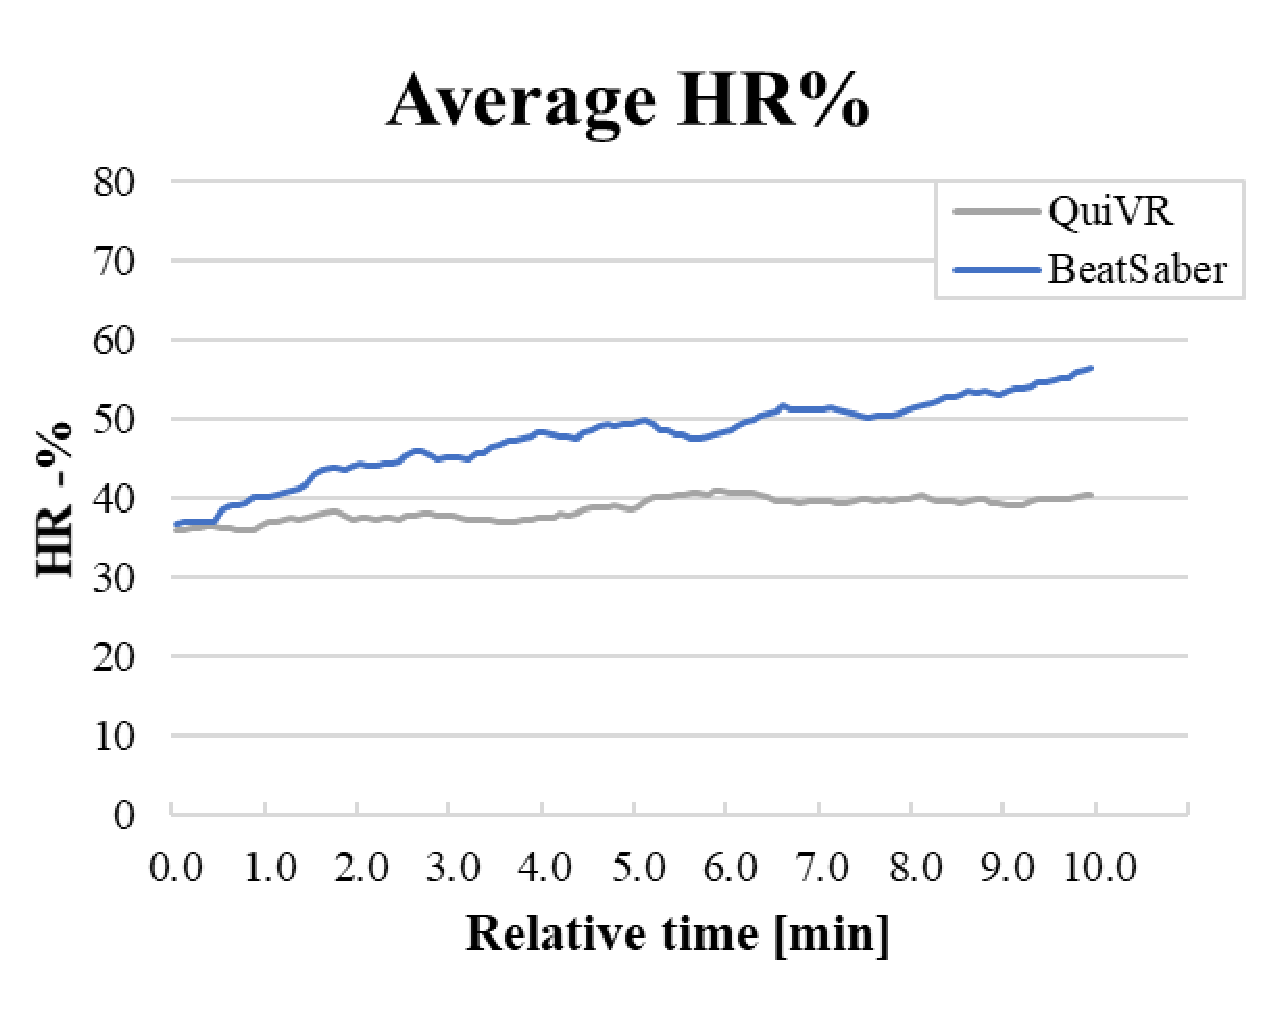
\includegraphics[width=0.45\textwidth]{heartrate}
    \caption
        {
            Average heart rates of participants at each game session.
        }
\end{figure}

\subsubsection{Movement data}

Test user’s movement data was collected using the capture program which was running 
parallel to the VR game. The program sampled the position and orientation data from 
all the three devices at a rate of 5 Hz. Each sample, including the current timestamp, 
was saved as a row to a result file. By calculating the displacement between each 
successive row, an estimate of the distance travelled by each device was obtained. 
The total distance was calculated by simply summing the travelled distance from all 
three devices. The total distance travelled by each user is shown in Figure 4. 

\begin{figure}
    \centering
    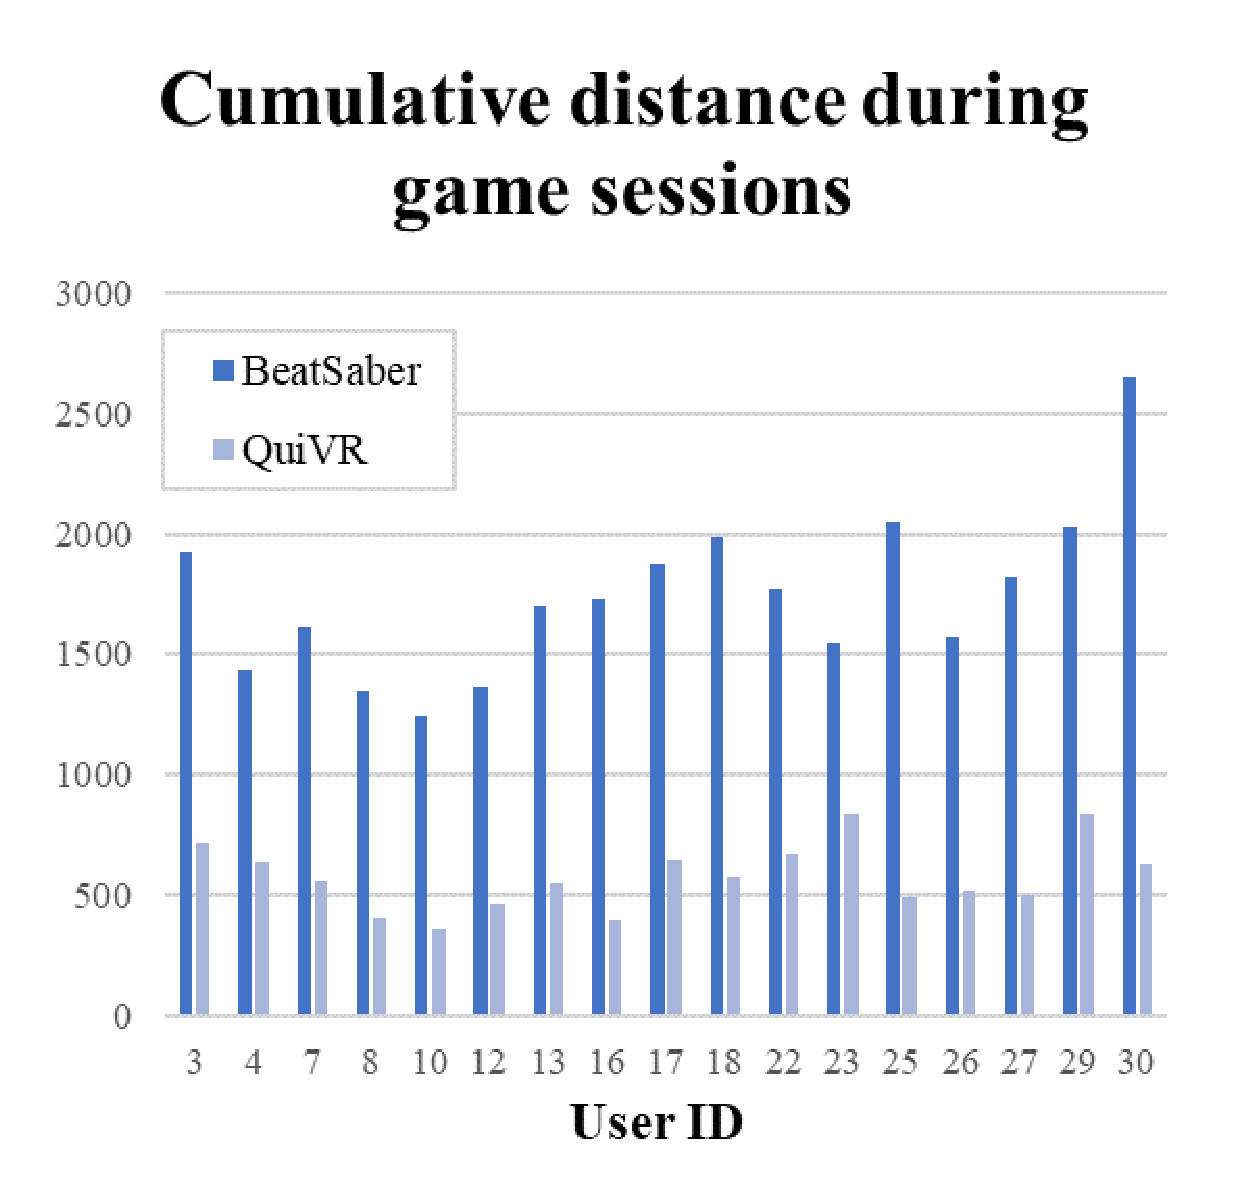
\includegraphics[width=0.45\textwidth]{motiondata}
    \caption
        {
            Movement data (total distance travelled) from each participants shown from different game sessions.
        }
\end{figure}

\subsection{Analysis of the data}

\subsubsection{Analysis of interviews}
Users did enjoy the game sessions. They said that gaming experience was fun, 
and some of them said that it was challenging. Participants rated BeatSaber 
slightly more intense game than QuiVR (Figure 2). As shown in Table I, 
participants ranked 4.6 out of five that they would play VR games for fun. 
Participants had neutral answers (2.6 out of five) to question, if VR games 
would encourage them to exercise more. Although, participants were more 
willing to recommend the VR games as an exercise form to someone else 
(3.4 out of five). Participants background with exercising or with videogames 
were irrelevant to the results.

The simulator sickness questionnaire did not show any critical results. 
Results are shown in Figure 3. User with an ID 12 had high weighted value of 
SSQ-D but the raw data includes only answers “slight” (value 1). SSQ-N 
results are shown higher peaks, but SSQ-N includes the weighted values 
from increasing sweating. Sweating is most likely caused by moving during 
games.

\subsubsection{Analysis of heart rate data}
\begin{table}[]
    \centering
    \caption
    {Average relative HR values before and after the game sessions. n=14}
    \begin{tabular}{cccccc} \hline
    &\multicolumn{2}{c}{Start}&\multicolumn{2}{c}{End}\\
    Game&Avg HR&STD&Avg HR&STD&Dif. HR\\\hline
    QuiVR&36&7&41&10&5\\
    BeatSaber&37&7&57&10&10 \\ \hline
    \end{tabular}
\end{table}

Average heart rate data from 14 participants (Table II) shows that in 
BeatSaber game session participants relative heart rates raised approximately 
20 percent, while in QuiVR heart rates stayed in the same. Twelve subjects 
reached the target HR zone of 50\% their maximum heart rate while playing 
BeatSaber. 

\subsubsection{Analysis of the movement data}

Users movements were detected during game sessions, and distance participant 
moved during game sessions were calculated. In Figure 5, it can be seen that 
users moved more while playing BeatSaber than QuiVR.

\section{DISCUSSION}
During the interviews, the subjects did not rank either game as being very 
intense, with QuiVR and BeatSaber receiving average scores of 2.3 and 3 out 
of five respectively. The subjects felt unsure if VR games could motivate 
them to exercise more. However, most viewed the experience positively and 
some could see themselves recommending VR games as exercise for someone 
else even if they felt they did not benefit from it themselves. Even VR 
equipment have become more frequent, they still are quite expensive and 
cannot be found in every home. This might be a reason participant did 
not see themselves playing VR exergames as an exercise purpose.

As can be seen from Figure 4. the heart rate in BeatSaber game raise 
during the whole game session and it probably have been raised higher 
if the game session had been continued more than 10 minutes. In QuiVR 
game session the heart rates of participant did not raised, and it is 
hard to predict if it has been raised if the game session has been longer.

It is confirmed with the movement data (Figure 5) that heart rates did 
not raise just because the game was excited. It can be seen clearly that 
participant had more movements when they played BeatSaber. 

In some cases when a person is playing a VR game, he/she experience 
cybersickness. One symptom of cybersickness is rising heart rate. To 
exclude the heart rate rising due to cybersickness, participant also 
had simulator sickness questionnaire by Kennedy et al. (1993). This 
questionnaire confirmed that no one of the test users had cybersickness. 
Used games, BeatSaber and QuiVR, are popular and one reason of that is 
their good quality.

\section{CONCLUSIONS}
Active VR games can raise the heart rate to levels comparable to 
normal exercise. The game with more relaxed gameplay did not manage 
to raise heart rate to similar levels. Although the participants viewed 
VR games in a positive light, the effects on exercise motivation are 
hard to gauge based on the small sample size and cross-sectional nature 
of our study. In the future it would be interesting to see how a VR 
based exercise regimen might affect exercise motivation in the long term.  

%\end{document}  % This is where a 'short' article might terminate

%ACKNOWLEDGMENTS are optional
\section{Acknowledgments}
We would like to thank to professor Timo Ojala who made this study 
possible by organizing the Ubiquitous Computing Fundamentals course. 
We would also like to thank course assistants Paula Alavesa and Aku Visuri. 
With the guidance from Alavesa and Visuri we were able to proceed this 
study. Especially we would like to thank all participants who were willing 
to give an hour of their time for this study.

\section{Contributions}
Kivelä, Oona: Design, performing an experiment, writing, presentation, analysis of results, recruit participant, project manager

Kuosmanen, Toni: Design, performing an experiment, experiment setup, coding, writing, presentation, analysis of results, recruit participants

Lämpsä, Timo: Design, performing an experiment

Mustajärvi, Leevi: Design, performing an experiment, experiment setup, writing, presentation, recruit participants

Soudunsaari, Joonas: Design, performing an experiment, experiment setup, recruit participants

%
% The following two commands are all you need in the
% initial runs of your .tex file to
% produce the bibliography for the citations in your paper.
\bibliographystyle{abbrv}
\bibliography{teamalpha}  
% You must have a proper ".bib" file
%  and remember to run:
% latex bibtex latex latex
% to resolve all references
%
% ACM needs 'a single self-contained file'!
%
%APPENDICES are optional
%\balancecolumns
\pagebreak
\appendix
%Appendix A
\section{Consent form}
\includepdf[pages={1}]{consent.pdf}
\end{document}
